\section{Results}

\subsection{Cluster Characteristics}

K-Means clustering identified three distinct farmer segments based on baseline skill profiles and training participation patterns. Segment 1 (low-skill) consists of farmers with uniformly low competencies across marketing, production management, and record-keeping, indicating limited readiness for advanced training. Segment 2 (moderate-skill) exhibits heterogeneous combinations of strengths and weaknesses, reflecting transitional capability profiles commonly observed in extension systems. Segment 3 (high-skill) comprises farmers with consistently strong baseline competencies and a higher likelihood of prior Smart Farmer participation. These patterns align with established findings on heterogeneous learning pathways in agricultural extension \citep{davis2012impact} and provide a structured basis for segment-aware training allocation.

\begin{figure}[t]
    \centering
    
\includegraphics[width=\linewidth]{figures/fig2_clusters.png}
    \caption{K-Means clustering results showing three farmer segments based on baseline skill profiles.}
    \label{fig:clusters}
\end{figure}

\subsection{Model Performance}

The Random Forest model achieved an $R^2$ of 0.132 under 5-fold cross-validation. Although modest, this level of explanatory power is consistent with the inherent stochasticity of human learning outcomes and the observational nature of the dataset \citep{ferreira2020mlagri}. Linear regression achieved a higher global $R^2$ (0.270), but its additive structure limits its ability to capture the non-linear and interaction effects revealed by SHAP. These results reinforce the role of the Random Forest not as a superior predictive model, but as a model capable of uncovering structural patterns necessary for explainability and rule extraction.

\subsection{Global SHAP Interpretation}

Global SHAP analysis highlights \textit{Avg Mkting} as the most influential predictor of skill improvement. The feature exhibits a non-monotonic pattern: farmers with high baseline marketing skills show both strong positive and negative SHAP values, suggesting the presence of ceiling effects in adult learning \citep{doran2017xai}. \textit{Avg ProdManage} and \textit{RiskPerception} also demonstrate substantial contributions, reflecting the importance of managerial readiness and behavioral attitudes. These findings indicate that both human capital and behavioral constraints jointly shape training outcomes.

\begin{figure}[t]
    \centering
    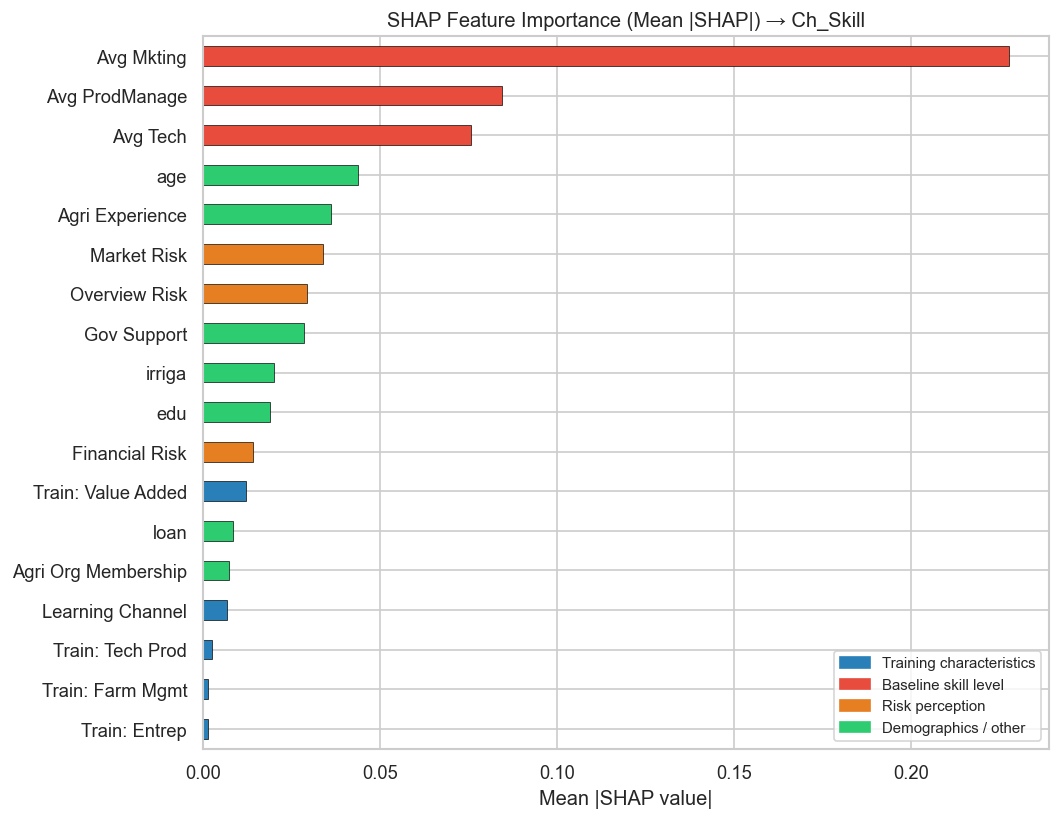
\includegraphics[width=\linewidth]{figures/fig3_importance.png}
    \caption{Global feature importance based on mean absolute SHAP values.}
    \label{fig:shap_importance}
\end{figure}

\begin{figure}[t]
    \centering
    
\includegraphics[width=\linewidth]{figures/fig4_shap.png}
    \caption{Global SHAP beeswarm plot showing non-linear and interaction effects across features.}
    \label{fig:shap_beeswarm}
\end{figure}

\subsection{Cluster-Level SHAP Analysis}

To examine heterogeneity in learning mechanisms, SHAP values were stratified by the three clusters. Low-skill farmers benefit primarily from foundational competencies, with \textit{All\_Skill} and \textit{Avg ProdManage} contributing positively to skill improvement. Moderate-skill farmers show strong sensitivity to marketing and production management, indicating that targeted reinforcement in these domains may yield substantial gains. High-skill farmers exhibit attenuated or negative SHAP contributions, consistent with saturation effects and limited room for measurable improvement. This cluster-stratified SHAP approach aligns with recent recommendations in agricultural XAI research \citep{ryo2022shap} and provides empirical justification for segment-aware training strategies.

\begin{figure*}[t]
    \centering
    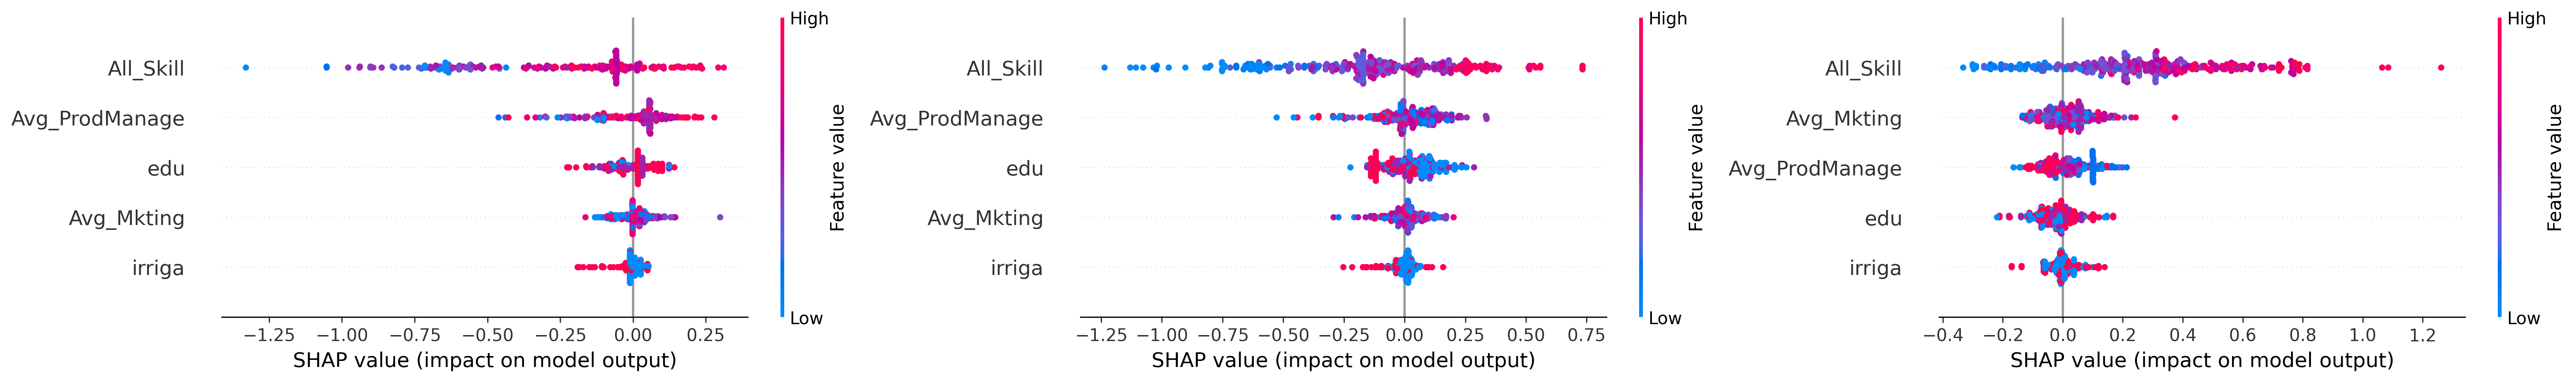
\includegraphics[width=\textwidth]{figures/fig4b_cluster_shap.png}
    \caption{Cluster-stratified SHAP profiles for low-, moderate-, and high-skill farmer segments.}
    \label{fig:cluster_shap}
\end{figure*}

\subsection{Surrogate Rule Extraction}

A surrogate decision tree (depth = 3) was fitted using SHAP-selected features to translate model behavior into transparent IF–THEN rules. The resulting rules highlight the importance of marketing capability, managerial readiness, and risk attitudes as key determinants of training effectiveness. For example, farmers with low baseline skills and high risk perception are consistently mapped to foundational training pathways, while those with stronger marketing and production management competencies are directed toward advanced or market-oriented interventions. These interpretable rules provide actionable guidance for extension officers and align with calls for transparent AI in agricultural DSS \citep{molnar2022interpretable}.

\begin{figure}[t]
    \centering
    
\includegraphics[width=\linewidth]{figures/fig5_rules.png}
    \caption{Surrogate decision tree summarizing segment-aware decision rules for training allocation.}
    \label{fig:rules}
\end{figure}
